\documentclass{beamer}

\usepackage[utf8]{inputenc}
\usepackage[T1]{fontenc}
\usepackage{listings}

%% Choose a theme from one of the following:
% AnnArbor, Antibes, Bergen, Berkeley, Berlin, Boadilla, boxes, CambridgeUS
% Copenhagen, Darmstadt, default, Dresden, Frankfurt, Goettingen, Hannover
% Ilmenau, JuanLesPins, Luebeck, Madrid, Malmoe, Marburg, Montpellier,
% PaloAlto, Pittsburgh, Rochester, Singapore, Szeged, Warsaw
%\usetheme{Warsaw}

\setbeamercovered{transparent}

\hypersetup{pdfpagelabels=true}

\lstset{ 
language=Python,
breaklines=true,   
basicstyle=\ttfamily,
keywordstyle=\color{keywordcolor},
        commentstyle={\color{commentcolor}\itshape},
        stringstyle={\color{stringcolor}\underbar},
        identifierstyle=\color{idcolor},numbers=left,
        xleftmargin=2em,framerule=0.8pt,
        stepnumber=1,frame=tlrb,showstringspaces=false,
        firstnumber=1,numberstyle=\ttfamily,backgroundcolor=\color{bg}}


%% Choose one of the following color themes or go with the default
% albatross, beaver, beetle, crane, default, dolphin, dove, fly
% lily, orchid, rose, seagull, seahorse sidebartab, structure
% whale, wolverine
\usecolortheme{dove}

\title[Sound Evolution] {Using genetic algorithms to evolve \emph{aesthetic} sounds.}
\subtitle{Humans as a fitness function}

\titlegraphic{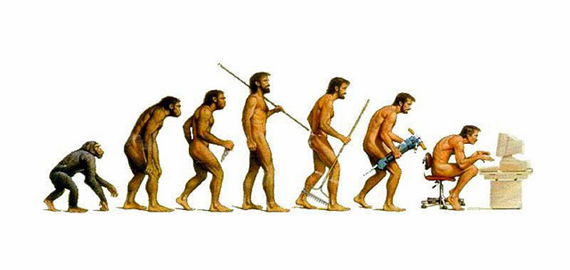
\includegraphics[height=3cm]{images/evolution}}

\author[Duncan, Matthias, Rafael, Mirko \& Stephan] { \\\texttt{..@bccn-berlin.de}} 
\date[SS 2010] {\today}

\pgfdeclareimage[height=0.8cm]{university-logo}{images/bccn_logo.png}
\logo{\pgfuseimage{university-logo}}

\beamerdefaultoverlayspecification{<1->}


\AtBeginSection[]{
	\begin{frame}%<beamer>
		\frametitle{outline}
		\tableofcontents[currentsection]
	\end{frame}
}


\begin{document}

\frame{\titlepage}

\section*{Outline}
\begin{frame}
  \frametitle{Outline}
  \tableofcontents[pausesections]
\end{frame}


\begin{frame}
	\frametitle{Duncan lutscht Schwaenze}
	\framesubtitle{in der Hoelle}
	
\end{frame}


\section{Background} % (fold)
\label{sg:sec:background}

\subsubsection{GP in general} % (fold)
\label{sg:ssub:gp_in_general}

\begin{frame}
	\frametitle{Genetic algorithms}
	\framesubtitle{the idea}
	
	\begin{itemize}
		\item<1-> use the principles of evolution (crossover, mutation, selection)
		to solve optimization problems
		\item<2-> this methods are successfully used in (engineering, robotics, network routing,
		automated joke generation) 
		\item<3-> main problem often to find and design a fitness function
	\end{itemize}
\end{frame}
% subsubsection gp_in_general (end)


\subsubsection{Inspiration for the Project} % (fold)
\label{sg:ssub:inspiration_for_the_project}

\begin{frame}
	\frametitle{Inspiration}
	\framesubtitle{GE in art}
	
	\begin{itemize}
		\item<1-> Synthesizer parameter fitting
		\item<2-> Image approximation (compression)
		\item<3-> Picbreeder
	\end{itemize}
\end{frame}

\begin{frame}
	\frametitle{Inspiration}
	\framesubtitle{Synthesizer parameter fitting}

	\begin{itemize}
		\item<1-> even if you know that a certain model is capable of performing a sound
		it might be hard to find the right parameters
		\item<2-> parameters could be found by using GP
		\item<3-> project website: \href{http://www.batuhanbozkurt.com/news/naturetoolkit-update-genetic-algorithms-and-parameter-estimation-for-supercollider}{www.batuhanbozkurt.com}
		\item<4-> \href{http://vimeo.com/7908757}{video at around 5:20}
	\end{itemize}
\end{frame}

\begin{frame}
	\frametitle{Inspiration}
	\framesubtitle{Image approximation (compression)}
	
	\begin{itemize}
		\item<1-> demo on: \href{http://alteredqualia.com/visualization/evolve/}{alteredqualia.com}
		\item<2-> gallery on: \href{http://rogeralsing.com/2008/12/11/genetic-gallery/}{rogeralsing.com}
	\end{itemize}
\end{frame}

\begin{frame}
	\frametitle{Inspiration}
	\framesubtitle{Picbreeder}
	
	Evolution of images by using people as a fitness function.
	\\
	\href{http://picbreeder.org/}{http://picbreeder.org/} 
\end{frame}


% subsubsection inspiration_for_the_project (end)
% section background (end)


\section{The idea} % (fold)
\label{sg:sec:the_idea}

\begin{frame}
	\frametitle{Problems}
	\framesubtitle{Technical problems}
	
	\begin{itemize}
		\item<1-> No objective measurement of aesthetics
		\item<2-> Huge search space
		\item<3-> Slow iterations
		\item<4-> Is an aesthetic result possible - even over time?
	\end{itemize}
	
\end{frame}

\begin{frame}
	\frametitle{The idea}
	\framesubtitle{A human fitness function}
	\begin{itemize}
		\item<1-> Web interface where people rate the fitness of individuals
		\item<2-> Loads of people needed
	\end{itemize}
	
\end{frame}

% section the_idea (end)


\section{The genome} % (fold)
\label{sg:sec:the_genome}

\begin{frame}
	\frametitle{The Genome}
	\framesubtitle{Tree structure}
	\begin{itemize}
		\item<1-> Genome often represented as tree
		\item<2-> Powerful algorithms on trees available
		\item<3-> Genetic operators easy to define on trees
	\end{itemize}
\end{frame}

\begin{frame}
	\frametitle{The Genome}
	\framesubtitle{Tree example}
	\begin{figure}[h]
		\centering
			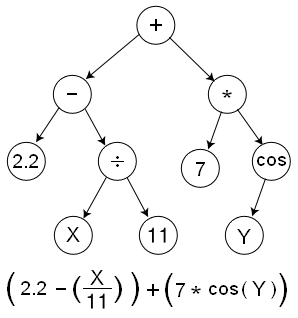
\includegraphics[width=0.6\textheight]{images/Genetic_Program_Tree.png}
		\caption{Tree representation of a mathematical expression}
		\label{sg:fig:images_Genetic_Program_Tree}
	\end{figure}
\end{frame}

\begin{frame}
	\frametitle{Operations on a tree}
	\framesubtitle{Genesis, crossover and mutations}
	\begin{description}
		\item<1->[Genesis] Syntactically valid random tree
		\item<2->[Mutation] replace branch by random tree
		\item<3->[Crossover] replace branch by branch of other tree
	\end{description}
\end{frame}


% section the_genome (end)


\section{Implementation} % (fold)
\begin{frame}
	\frametitle{Creating/ Changing/ Evolving Sounds}
	\begin{itemize}
	\item<1-> Python code 
	\item<2-> Git subversion system - for religious reasons
	\item<3-> All bow down to the great techie master Mirko
	\item<4-> Nose for testing 
	\item<5-> Lots of tests necessary for creating playable files (most time expended)
	\item<6-> Graph viz for visualization
         \end{itemize}

\end{frame}


\label{sg:sec:imple}

% section imple (end)

% NOTE here demonstration


\section{Outlook, many more ideas} % (fold)
\label{sg:sec:outlook_many_more_ideas}

 Failure of aesthetic aspect may stimulate search for elemental parameters.



% section outlook_many_more_ideas (end)

% TODO add a proper bibliography
%http://en.wikipedia.org/wiki/Computational_humor



\end{document}
